\documentclass[11pt]{article}
\usepackage{amsmath,amssymb}
\usepackage{booktabs}
\usepackage{graphicx}
\usepackage{longtable}
\usepackage{hyperref}
\usepackage[margin=1in]{geometry}
\usepackage{natbib}
% Generated by rfsrealloc.pipeline; do not edit.

\newcommand{\valabsorbableDrawdown}{2.0}
\newcommand{\valadditionalAB}{250}
\newcommand{\valadditionalBBD}{180}
\newcommand{\valadditionalExactRF}{766.8}
\newcommand{\valadditionalRF}{770}
\newcommand{\valadditionalRFReportedBasis}{760}
\newcommand{\valbankBaseline}{4.37}
\newcommand{\valbankOutFirstAllTwoZeroTwoSeven}{3.37}
\newcommand{\valbankOutFirstEqual}{3.01}
\newcommand{\valbankOutFirstSetTwo}{3.37}
\newcommand{\valbankOutSecondAllTwoZeroTwoSeven}{1.56}
\newcommand{\valbankOutSecondEqual}{1.57}
\newcommand{\valbankOutSecondSetTwo}{2.33}
\newcommand{\valbankRia}{3.6}
\newcommand{\valbtFirstTargetYear}{2021}
\newcommand{\valbtLastTargetYear}{2027}
\newcommand{\valbtMaeAllSecond}{1,003}
\newcommand{\valbtMaeEqual}{969}
\newcommand{\valbtNTargetYears}{7}
\newcommand{\valbtNYearsFullyUnknownEqual}{6}
\newcommand{\valbtUnknownAllSecondFirst}{160}
\newcommand{\valbtUnknownAllSecondSecond}{1,760}
\newcommand{\valbtUnknownEqualFirst}{960}
\newcommand{\valbtUnknownEqualSecond}{880}
\newcommand{\valbtUnknownShareAllFirst}{1.0}
\newcommand{\valbtUnknownShareAllSecond}{0.876}
\newcommand{\valbtUnknownShareAllSecondFirst}{0.139}
\newcommand{\valbtUnknownShareAllSecondSecond}{1.0}
\newcommand{\valbtUnknownShareEqual}{0.932}
\newcommand{\valbtUnknownShareEqualFirst}{0.66}
\newcommand{\valbtUnknownShareEqualSecond}{1.0}
\newcommand{\valcapBindsAnywhere}{no}
\newcommand{\valcapFirstAllTwoZeroTwoSeven}{5.36}
\newcommand{\valcapFirstEqual}{5.44}
\newcommand{\valcapFirstSetTwo}{5.36}
\newcommand{\valcapSecondAllTwoZeroTwoSeven}{5.56}
\newcommand{\valcapSecondEqual}{5.48}
\newcommand{\valcapSecondSetTwo}{5.4}
\newcommand{\valcarryoverUsedFirstAllTwoZeroTwoSeven}{4.37}
\newcommand{\valcarryoverUsedFirstEqual}{4.37}
\newcommand{\valcarryoverUsedFirstSetTwo}{4.37}
\newcommand{\valcarryoverUsedSecondAllTwoZeroTwoSeven}{3.37}
\newcommand{\valcarryoverUsedSecondEqual}{3.01}
\newcommand{\valcarryoverUsedSecondSetTwo}{3.37}
\newcommand{\valconfigHash}{f45a4a00633f4fe8}
\newcommand{\valconfigName}{paper}
\newcommand{\valcostRelFirstAllTwoZeroTwoSeven}{0.0}
\newcommand{\valcostRelFirstEqual}{0.37}
\newcommand{\valcostRelSecondAllTwoZeroTwoSeven}{0.79}
\newcommand{\valcostRelSecondEqual}{0.4}
\newcommand{\valcrossCheckBbdReduction}{0.31}
\newcommand{\valcrossCheckExtraExemptFuel}{5.83}
\newcommand{\valcrossCheckRfReduction}{0.9}
\newcommand{\valdStdPerOneZeroZeroMRinsFirst}{0.0578}
\newcommand{\valdStdPerOneZeroZeroMRinsSecond}{0.0584}
\newcommand{\valdeadlineDaysScenarioHypotheticalEarlyTwoZeroTwoSeven}{58}
\newcommand{\valdeadlineDaysScenarioHypotheticalLateTwoZeroTwoSeven}{61}
\newcommand{\valdeadlineDaysScenarioHypotheticalMidTwoZeroTwoSeven}{92}
\newcommand{\valdeadlineNotFinalized}{2027-12-01}
\newcommand{\valdeadlineScenarioHypotheticalEarlyTwoZeroTwoSeven}{2027-03-31}
\newcommand{\valdeadlineScenarioHypotheticalLateTwoZeroTwoSeven}{2027-12-01}
\newcommand{\valdeadlineScenarioHypotheticalMidTwoZeroTwoSeven}{2027-09-01}
\newcommand{\valdeficitFirstAllTwoZeroTwoSeven}{0.0}
\newcommand{\valdeficitFirstEqual}{0.0}
\newcommand{\valdeficitFirstSetTwo}{0.0}
\newcommand{\valdeficitSecondAllTwoZeroTwoSeven}{0.0}
\newcommand{\valdeficitSecondEqual}{0.0}
\newcommand{\valdeficitSecondSetTwo}{0.0}
\newcommand{\valdenominatorFirst}{173.02}
\newcommand{\valdenominatorSecond}{171.24}
\newcommand{\valdrawdownExcessOverAbsorbableAllSecond}{0.81}
\newcommand{\valdrawdownExcessOverAbsorbableEqual}{0.8}
\newcommand{\valdrawdownTwoYearsAllSecond}{2.81}
\newcommand{\valdrawdownTwoYearsEqual}{2.8}
\newcommand{\valdrawdownTwoYearsSetTwo}{2.04}
\newcommand{\valervoMismatchDescription}{2024 AB: computed 290, published 300}
\newcommand{\valervoMismatchMinVolumeBgal}{7.7836}
\newcommand{\valfuelErrorMaxPct}{6.0}
\newcommand{\valfuelErrorMeanPct}{2.19}
\newcommand{\valfuelErrorMinPct}{-3.71}
\newcommand{\valfuelErrorSdPct}{2.79}
\newcommand{\valimpliedDenominatorHiFirst}{173.024}
\newcommand{\valimpliedDenominatorHiSecond}{171.244}
\newcommand{\valimpliedDenominatorLoFirst}{173.019}
\newcommand{\valimpliedDenominatorLoSecond}{171.203}
\newcommand{\vallagTwoZeroTwoFourMedianYears}{0.64}
\newcommand{\vallagTwoZeroTwoFiveMedianYears}{0.66}
\newcommand{\vallagMaxYears}{3.85}
\newcommand{\vallagMedianYears}{1.64}
\newcommand{\vallagMinYears}{0.64}
\newcommand{\vallagYearsFirst}{2021}
\newcommand{\vallagYearsLast}{2025}
\newcommand{\vallaterShareTwoZeroTwoFourPct}{16.2}
\newcommand{\valmaxAbsResidualPoints}{0.0049}
\newcommand{\valmcDraws}{100,000}
\newcommand{\valmcseHeadlineRelative}{0.00224}
\newcommand{\valnCostChecked}{6}
\newcommand{\valnCostMatched}{6}
\newcommand{\valnDoubleEntryMismatches}{0}
\newcommand{\valnErvoChecked}{12}
\newcommand{\valnErvoMatched}{11}
\newcommand{\valnFrParsedValuesCompared}{156}
\newcommand{\valnFrParsedValuesMismatched}{0}
\newcommand{\valnFuelErrorsAll}{15}
\newcommand{\valnFuelErrorsProspective}{9}
\newcommand{\valnLagPetitions}{153}
\newcommand{\valnPendingTwoZeroTwoFive}{2}
\newcommand{\valnPendingTwoZeroTwoSix}{7}
\newcommand{\valnPendingTwoZeroTwoSeven}{4}
\newcommand{\valnProjYears}{10}
\newcommand{\valnProjYearsRealTime}{7}
\newcommand{\valnRevisionPairs}{7}
\newcommand{\valnSrervFloorCeilMatched}{6}
\newcommand{\valnSrervNearestMatched}{3}
\newcommand{\valnStandardsChangedByReportedBasis}{2}
\newcommand{\valnStandardsChecked}{32}
\newcommand{\valnStandardsMatched}{32}
\newcommand{\valnTableIVOneChecked}{12}
\newcommand{\valnTableIVOneMatched}{12}
\newcommand{\valnewRinsFirstAllTwoZeroTwoSeven}{22.45}
\newcommand{\valnewRinsFirstEqual}{22.81}
\newcommand{\valnewRinsFirstEqualMinusAllSecond}{0.36}
\newcommand{\valnewRinsFirstSetTwo}{22.45}
\newcommand{\valnewRinsSecondAbsDiffEqualAllSecond}{0.01}
\newcommand{\valnewRinsSecondAllTwoZeroTwoSeven}{24.42}
\newcommand{\valnewRinsSecondEqual}{24.41}
\newcommand{\valnewRinsSecondSetTwo}{23.65}
\newcommand{\valprojMaeHindsight}{476}
\newcommand{\valprojMaeHindsightPct}{42.1}
\newcommand{\valprojMaeRealTime}{1,090}
\newcommand{\valprojMaxAbsHindsight}{1,390}
\newcommand{\valrealizedMinusIntendedMeanFirstAllSecond}{0.458}
\newcommand{\valrealizedMinusIntendedMeanFirstEqual}{0.42}
\newcommand{\valrealizedMinusIntendedMeanSecondAllSecond}{0.518}
\newcommand{\valrealizedMinusIntendedMeanSecondEqual}{0.555}
\newcommand{\valrealizedMinusIntendedQZeroFiveFirstAllSecond}{-1.062}
\newcommand{\valrealizedMinusIntendedQZeroFiveFirstEqual}{-1.12}
\newcommand{\valrealizedMinusIntendedQZeroFiveSecondAllSecond}{-1.157}
\newcommand{\valrealizedMinusIntendedQZeroFiveSecondEqual}{-1.095}
\newcommand{\valrealizedMinusIntendedQNineFiveFirstAllSecond}{1.391}
\newcommand{\valrealizedMinusIntendedQNineFiveFirstEqual}{1.373}
\newcommand{\valrealizedMinusIntendedQNineFiveSecondAllSecond}{1.699}
\newcommand{\valrealizedMinusIntendedQNineFiveSecondEqual}{1.706}
\newcommand{\valrealizedMinusIntendedSdFirstAllSecond}{0.7}
\newcommand{\valrealizedMinusIntendedSdFirstEqual}{0.712}
\newcommand{\valrealizedMinusIntendedSdSecondAllSecond}{0.803}
\newcommand{\valrealizedMinusIntendedSdSecondEqual}{0.785}
\newcommand{\valreportedTwoZeroTwoFiveExemptedRvo}{1,750}
\newcommand{\valreportedTwoZeroTwoFiveExemptedVolume}{13,326}
\newcommand{\valreportedTwoZeroTwoFiveRatio}{0.9943}
\newcommand{\valreportedBasisMaxChangePoints}{0.01}
\newcommand{\valreportedBasisStdSecondAllSecond}{16.22}
\newcommand{\valreportedBasisStdSecondEqual}{16.00}
\newcommand{\valretroAllSecondScenarioHypotheticalEarlyTwoZeroTwoSeven}{0.085}
\newcommand{\valretroAllSecondScenarioHypotheticalLateTwoZeroTwoSeven}{0.748}
\newcommand{\valretroAllSecondScenarioHypotheticalMidTwoZeroTwoSeven}{0.414}
\newcommand{\valretroEqualScenarioHypotheticalEarlyTwoZeroTwoSeven}{0.542}
\newcommand{\valretroEqualScenarioHypotheticalLateTwoZeroTwoSeven}{0.874}
\newcommand{\valretroEqualScenarioHypotheticalMidTwoZeroTwoSeven}{0.707}
\newcommand{\valrevisionMeanAbsBRinsSecondAllSecond}{0.12}
\newcommand{\valrevisionMeanAbsFirstAllSecond}{0.0}
\newcommand{\valrevisionMeanAbsFirstEqual}{0.0344}
\newcommand{\valrevisionMeanAbsSecondAllSecond}{0.0695}
\newcommand{\valrevisionMeanAbsSecondEqual}{0.0347}
\newcommand{\valrevisionRatioMax}{1.014}
\newcommand{\valrevisionRatioMean}{0.95}
\newcommand{\valrevisionRatioMin}{0.828}
\newcommand{\valrevisionRatioSd}{0.067}
\newcommand{\valrvoFirstAllTwoZeroTwoSeven}{26.82}
\newcommand{\valrvoFirstEqual}{27.18}
\newcommand{\valrvoFirstSetTwo}{26.82}
\newcommand{\valrvoSecondAllTwoZeroTwoSeven}{27.79}
\newcommand{\valrvoSecondEqual}{27.42}
\newcommand{\valrvoSecondSetTwo}{27.02}
\newcommand{\valsensIndependentFuelRealizedMinusIntendedSdSecondAllSecond}{0.802}
\newcommand{\valsensIndependentFuelRealizedMinusIntendedSdSecondAllSecondIncreasePct}{-0.1}
\newcommand{\valsensIndependentFuelRealizedMinusIntendedSdSecondEqual}{0.784}
\newcommand{\valsensIndependentFuelRealizedMinusIntendedSdSecondEqualIncreasePct}{-0.1}
\newcommand{\valsensIndependentFuelRevisionMeanAbsFirstEqual}{0.0344}
\newcommand{\valsensIndependentFuelRevisionMeanAbsFirstEqualIncreasePct}{0.0}
\newcommand{\valsensIndependentFuelRevisionMeanAbsSecondAllSecond}{0.0695}
\newcommand{\valsensIndependentFuelRevisionMeanAbsSecondAllSecondIncreasePct}{0.0}
\newcommand{\valsensIndependentFuelStdSdFirstEqual}{0.037}
\newcommand{\valsensIndependentFuelStdSdFirstEqualIncreasePct}{0.0}
\newcommand{\valsensIndependentFuelStdSdSecondAllSecond}{0.0748}
\newcommand{\valsensIndependentFuelStdSdSecondAllSecondIncreasePct}{0.0}
\newcommand{\valsensUniformRealizedMinusIntendedSdSecondAllSecond}{0.82}
\newcommand{\valsensUniformRealizedMinusIntendedSdSecondAllSecondIncreasePct}{2.1}
\newcommand{\valsensUniformRealizedMinusIntendedSdSecondEqual}{0.789}
\newcommand{\valsensUniformRealizedMinusIntendedSdSecondEqualIncreasePct}{0.5}
\newcommand{\valsensUniformRevisionMeanAbsFirstEqual}{0.0509}
\newcommand{\valsensUniformRevisionMeanAbsFirstEqualIncreasePct}{48.0}
\newcommand{\valsensUniformRevisionMeanAbsSecondAllSecond}{0.1029}
\newcommand{\valsensUniformRevisionMeanAbsSecondAllSecondIncreasePct}{48.1}
\newcommand{\valsensUniformStdSdFirstEqual}{0.0588}
\newcommand{\valsensUniformStdSdFirstEqualIncreasePct}{58.9}
\newcommand{\valsensUniformStdSdSecondAllSecond}{0.1188}
\newcommand{\valsensUniformStdSdSecondAllSecondIncreasePct}{58.8}
\newcommand{\valshareABMINUSBBD}{0.0883}
\newcommand{\valshareBBD}{0.2399}
\newcommand{\valshareCB}{0.0541}
\newcommand{\valshareCONV}{0.6717}
\newcommand{\valshareOA}{0.0343}
\newcommand{\valsobolFuelRealizedFirstAllSecond}{1.0}
\newcommand{\valsobolFuelRealizedFirstEqual}{0.992}
\newcommand{\valsobolFuelRealizedSecondAllSecond}{0.979}
\newcommand{\valsobolFuelRealizedSecondEqual}{0.994}
\newcommand{\valsobolFuelStdFirstAllSecond}{0.0}
\newcommand{\valsobolFuelStdFirstEqual}{0.0}
\newcommand{\valsobolFuelStdSecondAllSecond}{0.0}
\newcommand{\valsobolFuelStdSecondEqual}{0.0}
\newcommand{\valsobolRevisionRealizedFirstAllSecond}{0.0}
\newcommand{\valsobolRevisionRealizedFirstEqual}{0.008}
\newcommand{\valsobolRevisionRealizedSecondAllSecond}{0.021}
\newcommand{\valsobolRevisionRealizedSecondEqual}{0.006}
\newcommand{\valsobolRevisionStdFirstAllSecond}{0.0}
\newcommand{\valsobolRevisionStdFirstEqual}{1.0}
\newcommand{\valsobolRevisionStdSecondAllSecond}{1.0}
\newcommand{\valsobolRevisionStdSecondEqual}{1.0}
\newcommand{\valstdMeanFirstAllSecond}{15.495}
\newcommand{\valstdMeanFirstEqual}{15.692}
\newcommand{\valstdMeanSecondAllSecond}{16.177}
\newcommand{\valstdMeanSecondEqual}{15.978}
\newcommand{\valstdQZeroFiveFirstAllSecond}{15.495}
\newcommand{\valstdQZeroFiveFirstEqual}{15.624}
\newcommand{\valstdQZeroFiveSecondAllSecond}{16.039}
\newcommand{\valstdQZeroFiveSecondEqual}{15.909}
\newcommand{\valstdQNineFiveFirstAllSecond}{15.495}
\newcommand{\valstdQNineFiveFirstEqual}{15.745}
\newcommand{\valstdQNineFiveSecondAllSecond}{16.284}
\newcommand{\valstdQNineFiveSecondEqual}{16.032}
\newcommand{\valstdSdFirstAllSecond}{0.0}
\newcommand{\valstdSdFirstEqual}{0.037}
\newcommand{\valstdSdSecondAllSecond}{0.0748}
\newcommand{\valstdSdSecondEqual}{0.0374}
\newcommand{\valstepAllSecondBRinsSecond}{0.77}
\newcommand{\valstepEqualBRinsFirst}{0.38}
\newcommand{\valstepEqualBRinsSecond}{0.38}
\newcommand{\valstepFirstEqual}{0.223}
\newcommand{\valstepSecondAllSecond}{0.45}
\newcommand{\valstepSecondEqual}{0.225}

\graphicspath{{../paper/figures/}}
\newcommand{\commentdate}{November 24, 2026}
\title{Technical Attachment to the Comment of Avin Gupta on Docket ID No. EPA-HQ-OAR-2024-0505 (Document EPA-HQ-OAR-2024-0505-0951)\\[0.5em]\large Exact reconstruction of the 2026--2027 percentage standards, uncertainty propagation and evaluation of reallocation timing rules}
\author{Avin Gupta, individual researcher (\texttt{iamavingupta@gmail.com})}
\date{\commentdate}
\begin{document}
\maketitle

\section{Purpose and scope}
This attachment documents the methods, data and results behind the accompanying comment. It is a condensed version of a preprint prepared for release; every number is generated by the repository \texttt{rfs-sre-reallocation} (package \texttt{rfsrealloc}) from the public record, with the configuration identified by hash \valconfigHash{}. Nothing here addresses legal authority (C-2) or infers prices.

\section{Data}
Inputs were transcribed from the docket calculation memoranda \citep{docket_0789,docket_0790,docket_0956}, the proposed rule \citep{fr_2026_21155}, the Set~2 rule \citep{fr_2026_06275} and its Regulatory Impact Analysis \citep{ria_420r26011}, EPA's SRE decision documents \citep{epa_420r25010,epa_420r25013,epa_420r26004,epa_420r26017}, the Federal Register notices of those decisions, the input tables of every annual standards rule since 2011, the eCFR text of 40~CFR~80.1405, 80.1427 and 80.1451 \citep{ecfr_80_1405,ecfr_80_1427,ecfr_80_1451}, and EPA's public data tables for small refinery exemptions and renewable volume obligations \citep{epa_sre_dashboard,epa_rvo_dashboard}. Each value carries a page or table citation and was entered twice independently (\valnDoubleEntryMismatches{} mismatches); the Federal Register tables were also parsed by code from the XML and compared with the transcription (\valnFrParsedValuesCompared{} values, \valnFrParsedValuesMismatched{} mismatches). Table~\ref{tab:inputs} lists the 2026--2027 inputs.

\begin{table}[htbp]
\centering
\caption{Inputs to the 2026--2027 percentage-standard equations (billion gallons; required volumes in billion gallon-RINs), as published in the docket calculation memorandum.}
\label{tab:inputs}
\footnotesize
\begin{tabular}{lrrr}
\toprule
Term & 2026 & 2027 & Source \\
\midrule
D & 60.46 & 59.72 & EPA-HQ-OAR-2024-0505-0789, p.~1 \\
DE & 3.20 & 3.20 & EPA-HQ-OAR-2024-0505-0789, p.~1 \\
G & 140.07 & 139.18 & EPA-HQ-OAR-2024-0505-0789, p.~1 \\
GE & 4.35 & 4.35 & EPA-HQ-OAR-2024-0505-0789, p.~1 \\
RD & 5.11 & 5.26 & EPA-HQ-OAR-2024-0505-0789, p.~1 \\
RFV\textsubscript{AB} & 10.82 & 10.98 & EPA-HQ-OAR-2024-0505-0789, p.~1 \\
RFV\textsubscript{BBD} & 8.86 & 8.95 & EPA-HQ-OAR-2024-0505-0789, p.~1 \\
RFV\textsubscript{CB} & 1.36 & 1.43 & EPA-HQ-OAR-2024-0505-0789, p.~1 \\
RFV\textsubscript{RF} & 25.82 & 25.98 & EPA-HQ-OAR-2024-0505-0789, p.~1 \\
RG & 14.85 & 14.85 & EPA-HQ-OAR-2024-0505-0789, p.~1 \\
\bottomrule
\end{tabular}
\end{table}


\section{Methods}
\paragraph{Percentage standards.} 40~CFR~80.1405(c) (91~FR~16488):
$\mathrm{Std}_{X,i} = 100\,(\mathrm{RFV}_{X,i} + \mathrm{SRERV}_{X,i}) / [(G_i - RG_i) - GE_i + (D_i - RD_i) - DE_i]$, with no cellulosic reallocation volume; evaluated in exact rational arithmetic and rounded half-up to two decimals.
\paragraph{Reallocation volumes.} $\mathrm{ERVO}_{X,y} = \mathrm{Std}_{X,y}F_y/100$ rounded to 10~million RINs; Set~2 volumes are 0.7 times (all of 2023 plus half of 2024) for 2026, rounded down, and 0.7 times (half of 2024 plus all of 2025) for 2027, rounded up. The additional 2025 obligation is the rounded actual obligation (13.38 billion gallons times the 2025 standards) minus the projected obligation. A share $w$ goes to 2026 and $1-w$ to 2027; $w=1/2$ and $w=0$ are the two co-proposed approaches.
\paragraph{Uncertainty.} Revision ratio $r$ (reported over petition-based obligation) from \valnRevisionPairs{} compliance years; fuel-use error (log of reported over projected non-renewable gasoline-plus-diesel volume) from \valnFuelErrorsProspective{} rules in place by the middle of the compliance year and not later revised, by lead time; decision lags from \valnLagPetitions{} petitions. Monte Carlo with \valmcDraws{} draws (seeded, worker-independent); Sobol indices by Saltelli sampling with bootstrap intervals. The relative Monte Carlo standard error of the headline quantity is \valmcseHeadlineRelative{}.
\paragraph{Timing metrics.} Step size, standard deviation, expected absolute revision, and retroactive share $w f_{2026}(t) + (1-w) f_{2027}(t)$ for hypothetical effective dates $t$.
\paragraph{Backtest.} Error of the three-year-average projection by year; share of the amount a fixed rule would reallocate to a receiving year that was undecided when that year's standard was set.
\paragraph{Carryover accounting.} 40~CFR~80.1427 cap of 20~percent and one-year deficit carryforward; generation assumed equal to the volume requirement; bank entering 2026 equal to EPA's effective 2024 carryover (\valbankRia{} billion RINs) plus 0.77 billion RINs; accounting identity checked each year; deadlines from 40~CFR~80.1451(f).

\section{Results}

\subsection{Reconstruction}\label{sec:recon}
\valnStandardsMatched{} of \valnStandardsChecked{} published standards reproduce exactly (Table~\ref{tab:reconstruction}; Figure~\ref{fig:residuals}); denominators \valdenominatorFirst{} and \valdenominatorSecond{} billion gallons; additional obligation \valadditionalBBD{}/\valadditionalAB{}/\valadditionalRF{} million RINs; all \valnTableIVOneChecked{} Table~IV-1 volumes and all \valnCostChecked{} Table~VI-1 RIN-cost rows reproduce. Set~2 reallocation volumes require floor (2026) and ceiling (2027) rounding (\valnSrervFloorCeilMatched{} of 6; the rule stated in the note to Table~IV-1 of the proposal, applied to the printed obligations, \valnSrervNearestMatched{} of 6). Exempted-obligation cells: \valnErvoMatched{} of \valnErvoChecked{} reproduce from printed values (exception: \valervoMismatchDescription{} million RINs). On the reported-data basis (\valreportedTwoZeroTwoFiveExemptedRvo{} million RINs, ratio \valreportedTwoZeroTwoFiveRatio), \valnStandardsChangedByReportedBasis{} standards change, each by \valreportedBasisMaxChangePoints{} points (2027 total renewable fuel: \valreportedBasisStdSecondEqual{} equal split, \valreportedBasisStdSecondAllSecond{} 2027 approach).

\begin{table}[htbp]
\centering
\caption{Reconstructed percentage standards (exact value and published two-decimal value) for the Set 2 rule and the two co-proposed alternatives.}
\label{tab:reconstruction}
\footnotesize
\begin{tabular}{lrrrrrrr}
\toprule
Alternative & Year & Category & Num. (bn RINs) & Den. (bn gal) & Exact (\%) & Publ. (\%) & Match \\
\midrule
Set 2 rule & 2026 & CB & 1.36 & 173.02 & 0.7860 & 0.79 & yes \\
Set 2 rule & 2026 & BBD & 9.07 & 173.02 & 5.2422 & 5.24 & yes \\
Set 2 rule & 2026 & AB & 11.10 & 173.02 & 6.4154 & 6.42 & yes \\
Set 2 rule & 2026 & RF & 26.81 & 173.02 & 15.4953 & 15.50 & yes \\
Set 2 rule & 2027 & CB & 1.43 & 171.24 & 0.8351 & 0.84 & yes \\
Set 2 rule & 2027 & BBD & 9.20 & 171.24 & 5.3726 & 5.37 & yes \\
Set 2 rule & 2027 & AB & 11.32 & 171.24 & 6.6106 & 6.61 & yes \\
Set 2 rule & 2027 & RF & 27.02 & 171.24 & 15.7790 & 15.78 & yes \\
Equal reallocation & 2026 & CB & 1.36 & 173.02 & 0.7860 & 0.79 & yes \\
Equal reallocation & 2026 & BBD & 9.16 & 173.02 & 5.2942 & 5.29 & yes \\
Equal reallocation & 2026 & AB & 11.22 & 173.02 & 6.4848 & 6.48 & yes \\
Equal reallocation & 2026 & RF & 27.19 & 173.02 & 15.7149 & 15.71 & yes \\
Equal reallocation & 2027 & CB & 1.43 & 171.24 & 0.8351 & 0.84 & yes \\
Equal reallocation & 2027 & BBD & 9.29 & 171.24 & 5.4251 & 5.43 & yes \\
Equal reallocation & 2027 & AB & 11.45 & 171.24 & 6.6865 & 6.69 & yes \\
Equal reallocation & 2027 & RF & 27.41 & 171.24 & 16.0068 & 16.01 & yes \\
2027 reallocation & 2026 & CB & 1.36 & 173.02 & 0.7860 & 0.79 & yes \\
2027 reallocation & 2026 & BBD & 9.07 & 173.02 & 5.2422 & 5.24 & yes \\
2027 reallocation & 2026 & AB & 11.10 & 173.02 & 6.4154 & 6.42 & yes \\
2027 reallocation & 2026 & RF & 26.81 & 173.02 & 15.4953 & 15.50 & yes \\
2027 reallocation & 2027 & CB & 1.43 & 171.24 & 0.8351 & 0.84 & yes \\
2027 reallocation & 2027 & BBD & 9.38 & 171.24 & 5.4777 & 5.48 & yes \\
2027 reallocation & 2027 & AB & 11.57 & 171.24 & 6.7566 & 6.76 & yes \\
2027 reallocation & 2027 & RF & 27.79 & 171.24 & 16.2287 & 16.23 & yes \\
\bottomrule
\end{tabular}
\end{table}


\subsection{Uncertainty propagation}
Sensitivity \valdStdPerOneZeroZeroMRinsFirst{} (2026) and \valdStdPerOneZeroZeroMRinsSecond{} (2027) points per 100~million RINs. Standard deviations of the total renewable fuel standard: equal split \valstdSdFirstEqual{} (2026) and \valstdSdSecondEqual{} (2027); 2027 approach \valstdSdSecondAllSecond{} (2027). Expected absolute revision: \valrevisionMeanAbsFirstEqual{} per year (equal split), \valrevisionMeanAbsSecondAllSecond{} (2027 approach). Realized-minus-intended obligation (fuel-use error): standard deviation \valrealizedMinusIntendedSdSecondEqual{} billion RINs, mean \valrealizedMinusIntendedMeanSecondAllSecond{}, 5--95~percent range \valrealizedMinusIntendedQZeroFiveSecondAllSecond{} to \valrealizedMinusIntendedQNineFiveSecondAllSecond{} (2027 approach, 2027). Sobol total-order index of the fuel-use error for realized 2027 RINs: \valsobolFuelRealizedSecondEqual{}. Table~\ref{tab:uncertainty} lists the empirical distributions.

\begin{table}[htbp]
\centering
\caption{Empirical distributions used in the uncertainty model (EPA decision documents and public data tables).}
\label{tab:uncertainty}
\footnotesize
\begin{tabular}{lrrrrrr}
\toprule
Quantity & n & Mean & SD & Min & Max & Basis \\
\midrule
Exemption revision ratio (reported / petition-based) & 7 & 0.950 & 0.067 & 0.828 & 1.014 & decisions; SRE-1 \\
Fuel-use ratio (reported / projected), prospective rules & 9 & 1.022 & 0.028 & 0.963 & 1.060 & RVO Table 1 \\
Decision lag after year end (years), 2021--2025 petitions & 153 & 1.718 & 1.110 & 0.641 & 3.852 & SRE-3 \\
\bottomrule
\end{tabular}
\end{table}


\subsection{Timing trade-offs}
Steps: equal split \valstepFirstEqual{} (2026) and \valstepSecondEqual{} (2027) points; 2027 approach \valstepSecondAllSecond{} (2027). Retroactive share for hypothetical effective dates February~1, June~1 and October~1, 2027: equal split \valretroEqualScenarioHypotheticalEarlyTwoZeroTwoSeven{}, \valretroEqualScenarioHypotheticalMidTwoZeroTwoSeven{}, \valretroEqualScenarioHypotheticalLateTwoZeroTwoSeven{}; 2027 approach \valretroAllSecondScenarioHypotheticalEarlyTwoZeroTwoSeven{}, \valretroAllSecondScenarioHypotheticalMidTwoZeroTwoSeven{}, \valretroAllSecondScenarioHypotheticalLateTwoZeroTwoSeven{}.

\subsection{Compliance deadlines}\label{sec:deadlines}
2026 compliance reporting deadline under 40~CFR~80.1451(f)(1)(i)(C): \valdeadlineScenarioHypotheticalEarlyTwoZeroTwoSeven{} (effective February~1, 2027; \valdeadlineDaysScenarioHypotheticalEarlyTwoZeroTwoSeven{} days after the effective date), \valdeadlineScenarioHypotheticalMidTwoZeroTwoSeven{} (effective June~1, 2027; \valdeadlineDaysScenarioHypotheticalMidTwoZeroTwoSeven{} days), \valdeadlineScenarioHypotheticalLateTwoZeroTwoSeven{} (effective October~1, 2027; \valdeadlineDaysScenarioHypotheticalLateTwoZeroTwoSeven{} days); \valdeadlineNotFinalized{} if neither finalized nor withdrawn within twelve months.

\subsection{Backtest}
Three-year-average projection: mean absolute error \valprojMaeHindsight{} million RINs (\valprojMaeHindsightPct{}~percent), maximum \valprojMaxAbsHindsight{}, over \valnProjYears{} years. Decision lags (2021--2025 petitions, $n=\valnLagPetitions$): median \vallagMedianYears{} years, range \vallagMinYears{}--\vallagMaxYears{}; 2025 petitions \vallagTwoZeroTwoFiveMedianYears{} years. Undecided share of reallocated amounts at the time the receiving year's standard was set: one in \valbtNYearsFullyUnknownEqual{} of \valbtNTargetYears{} receiving years (\valbtFirstTargetYear{}--\valbtLastTargetYear); for 2026, \valbtUnknownShareEqualFirst{} ($w=1/2$) and \valbtUnknownShareAllSecondFirst{} ($w=0$). Pending petitions at the data cut-off: \valnPendingTwoZeroTwoFive{} (2025), \valnPendingTwoZeroTwoSix{} (2026), \valnPendingTwoZeroTwoSeven{} (2027).

\subsection{Carryover accounting}
Baseline bank \valbankBaseline{} billion RINs. Obligations: 2026 \valrvoFirstSetTwo{} (existing), \valrvoFirstEqual{} (equal split); 2027 \valrvoSecondSetTwo{}, \valrvoSecondEqual{}, \valrvoSecondAllTwoZeroTwoSeven{}. New RINs required: 2026 \valnewRinsFirstSetTwo{}/\valnewRinsFirstEqual{}/\valnewRinsFirstAllTwoZeroTwoSeven{}; 2027 \valnewRinsSecondSetTwo{}/\valnewRinsSecondEqual{}/\valnewRinsSecondAllTwoZeroTwoSeven{}. Bank at end of 2027: \valbankOutSecondSetTwo{}/\valbankOutSecondEqual{}/\valbankOutSecondAllTwoZeroTwoSeven{}; two-year drawdown \valdrawdownTwoYearsSetTwo{}/\valdrawdownTwoYearsEqual{}/\valdrawdownTwoYearsAllSecond{} against \valabsorbableDrawdown{} judged absorbable in the Set~2 rule. Cap binds: \valcapBindsAnywhere{}. Table~\ref{tab:accounting} gives the full accounting.

\begin{table}[htbp]
\centering
\caption{Carryover-RIN accounting (billion RINs) under each alternative, assuming new RIN generation equal to the volume requirement and the baseline bank.}
\label{tab:accounting}
\footnotesize\setlength{\tabcolsep}{4pt}
\begin{tabular}{lrrrrrrr}
\toprule
Alternative & Year & Obligation & Bank in & 20\% cap & Carryover used & New RINs required & Bank out \\
\midrule
Set 2 rule & 2026 & 26.82 & 4.37 & 5.36 & 4.37 & 22.45 & 3.37 \\
Set 2 rule & 2027 & 27.02 & 3.37 & 5.40 & 3.37 & 23.65 & 2.33 \\
Equal reallocation & 2026 & 27.18 & 4.37 & 5.44 & 4.37 & 22.81 & 3.01 \\
Equal reallocation & 2027 & 27.42 & 3.01 & 5.48 & 3.01 & 24.41 & 1.57 \\
2027 reallocation & 2026 & 26.82 & 4.37 & 5.36 & 4.37 & 22.45 & 3.37 \\
2027 reallocation & 2027 & 27.79 & 3.37 & 5.56 & 3.37 & 24.42 & 1.56 \\
\bottomrule
\end{tabular}
\end{table}


\subsection{RIN-cost reproduction}
Table~VI-1 RIN costs reproduce (\valnCostMatched{} of \valnCostChecked); impact relative to existing standards \valcostRelFirstEqual{}/\valcostRelSecondEqual{} cents per gallon (equal split, 2026/2027) and 0.00/\valcostRelSecondAllTwoZeroTwoSeven{} (2027 approach), matching the docket memorandum.

\section{Figures}
\begin{figure}[htbp]\centering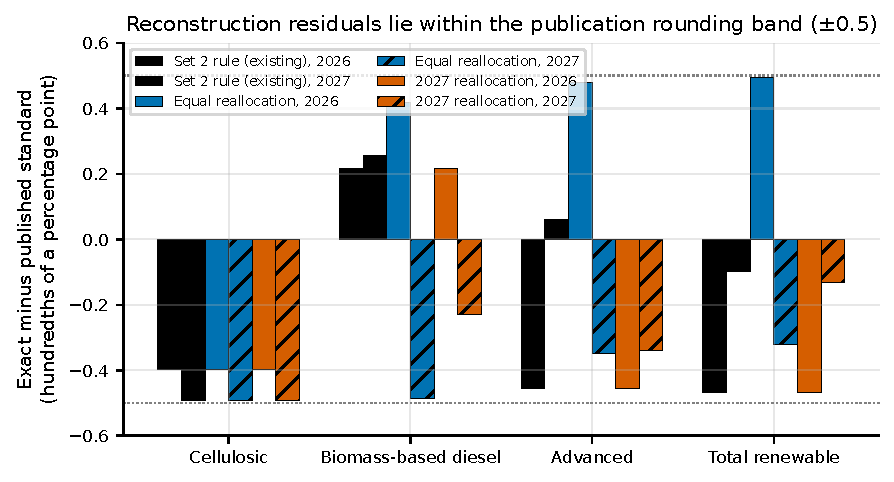
\includegraphics[width=\textwidth]{fig2_residuals}\caption{Reproduction residuals (exact minus published standard, hundredths of a point). Observed/published basis.}\label{fig:residuals}\end{figure}
\begin{figure}[htbp]\centering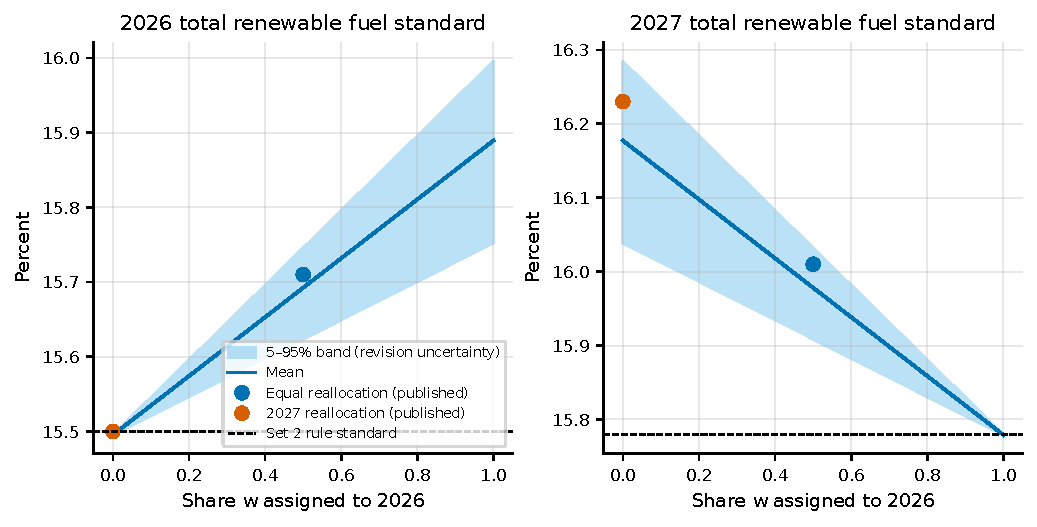
\includegraphics[width=\textwidth]{fig3_bands}\caption{Standards as a function of the timing share $w$ with the 5--95~percent band from the empirical revision distribution (modelled); published values as points.}\label{fig:bands}\end{figure}
\begin{figure}[htbp]\centering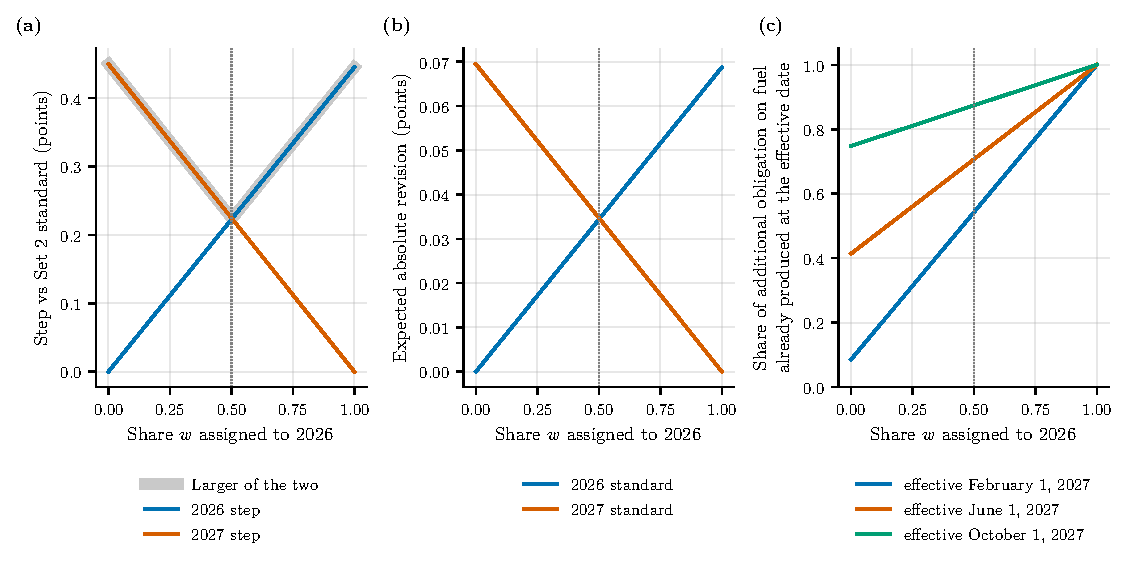
\includegraphics[width=\textwidth]{fig4_tradeoff}\caption{Timing trade-offs: step size, expected absolute revision, and retroactive share under hypothetical effective dates.}\label{fig:tradeoff}\end{figure}
\begin{figure}[htbp]\centering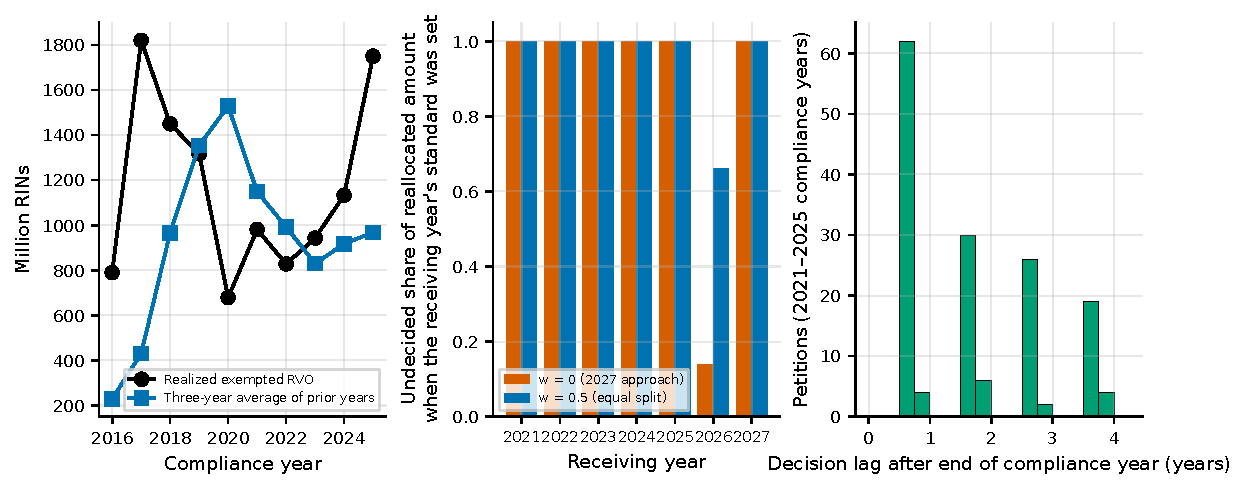
\includegraphics[width=\textwidth]{fig5_backtest}\caption{Historical backtest: realized exempted obligations and three-year-average projections; undecided share of reallocated amounts by receiving year; decision lags. Observed EPA record.}\label{fig:backtest}\end{figure}
\begin{figure}[htbp]\centering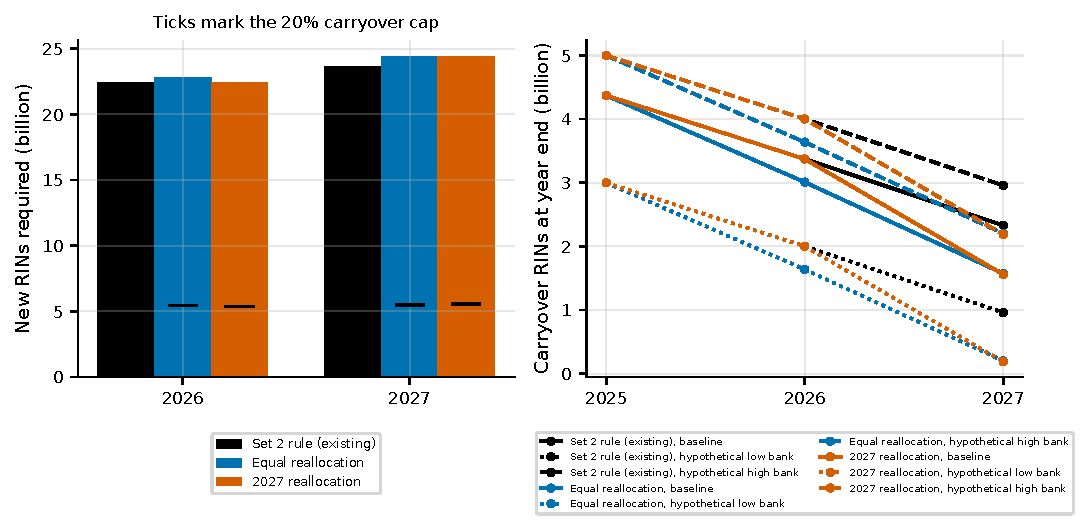
\includegraphics[width=\textwidth]{fig6_carryover}\caption{Carryover accounting under stated assumptions; non-baseline bank sizes are hypothetical scenarios.}\label{fig:carryover}\end{figure}

\section{Validation levels}
Numerical correctness: unit and property-based tests (reproduction of every published value; positivity, monotonicity, exact-versus-float agreement, rounding, conservation, accounting identity). Model verification: double entry, code-parsed Federal Register tables, eCFR table, linearised variance check. Empirical validity: distributions are historical; no prediction claimed. Regulatory applicability: mapped to C-1 and C-3 in the comment.

\section{Repository}
Code (BSD 3-Clause), transcribed data (CC~BY~4.0) and raw downloads with SHA-256 checksums are in the repository \texttt{rfs-sre-reallocation}; a single command regenerates all results, figures and tables. An archived release identifier will be cited when the repository is made public.

\bibliographystyle{plainnat}
\bibliography{../paper/references}
\end{document}
